% \tikzexternaldisable

\tikzsetnextfilename{fig-cubic-standard}
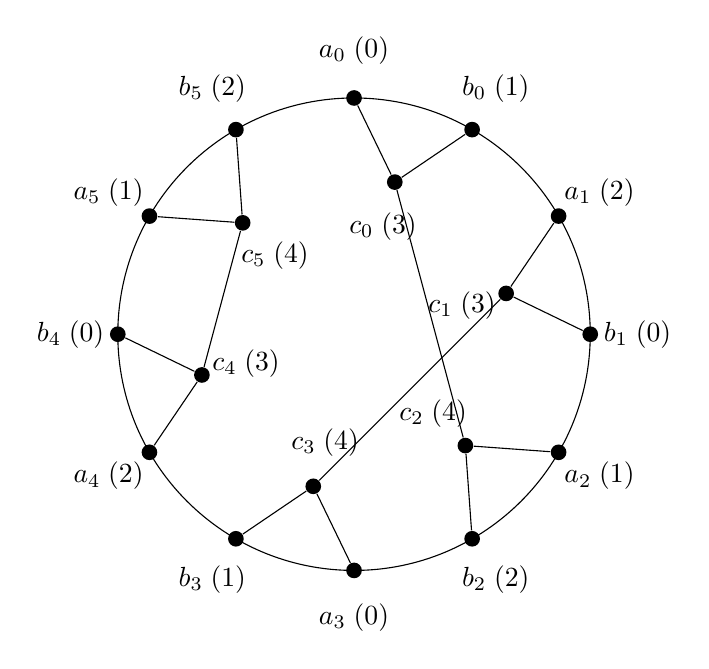
\begin{tikzpicture}[scale=1, transform shape,
    vertex/.style={circle, fill=black, inner sep=2pt}
]

% Círculo exterior
\draw (0,0) circle (3cm);

% Vértices a_i, b_i
\foreach \i/\name/\col in {
    0/$a_0$/0, 1/$b_0$/1, 2/$a_1$/2, 3/$b_1$/0,
    4/$a_2$/1, 5/$b_2$/2, 6/$a_3$/0, 7/$b_3$/1,
    8/$a_4$/2, 9/$b_4$/0, 10/$a_5$/1, 11/$b_5$/2}
{
    \node[vertex] (v\i) at ({90-30*\i}:3) {};
    \node [shift=({90-30*\i}:0.6)] at (v\i) {\name\;(\col)};
}

% Vértices c_i
\foreach \i/\name/\col in {
    0/$c_0$/3, 1/$c_1$/3, 2/$c_2$/4,
    3/$c_3$/4, 4/$c_4$/3, 5/$c_5$/4}
{
    \node[vertex] (c\i) at ({75-60*\i}:2) {};
    \node [shift=({75-60*\i}:-0.58)] at (c\i) {\name\;(\col)};
}

% Aristas a_i-c_i y b_i-c_i
\foreach \i in {0,...,5}
{
    \pgfmathtruncatemacro{\a}{2*\i}
    \pgfmathtruncatemacro{\b}{2*\i+1}
    \draw (v\a)--(c\i)--(v\b);
}

% Aristas del matching M
\draw (c0)--(c2);
\draw (c1)--(c3);
\draw (c4)--(c5);

\end{tikzpicture}